\section{Transposition Ciphers}

	We've taken a look at substitution ciphers, when letters are replaced by other letters. Another common type of cipher is a \textit{transposition} cipher, where the letters stay the same, but are reordered in the ciphertext.

\subsection{Scytale}

	\begin{figure}[h]
		\centering
		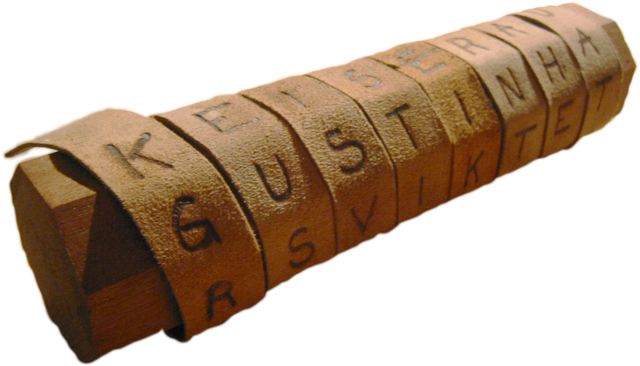
\includegraphics[width=0.7\linewidth]{McrRaspJam/016_Ciphers/3_transposition/Scytale}
		\caption{A scytale device}
		\label{fig:scytale}
	\end{figure}
	
	The scytale dates back to Ancient Greece and Sparta, and is a very simple to use device for encrypting methods.
	
	A person wishing to encrypt a message would simply wrap a long strip of parchment around the cylinder of the scytale and write their message across in rows. When unwrapped, the message would appear to be nonsense.
	
	\begin{itemize}[nosep]
		\item The scytale has a cryptographic key, what is it?
	\end{itemize}
	
	\begin{figure}[h]
		\centering
		
		\begin{tabular}{c|c|c|c|c}
			w & e & a & r & e \\ 
			\hline 
			d & i & s & c & o \\ 
			\hline 
			v & e & r & e & d \\ 
			\hline 
			h & e & l & p &  \\
		\end{tabular}
	
		\vspace{4pt}
		
		\begin{tabular}{ccccccccccccccccccc}
			w & d & v & h & e & i & e & e & a & s & r & l & r & c & e & p & e & o & d \\ 
		\end{tabular} 
	
		\caption{A scytale plaintext, and its unwrapped ciphertext}
		\label{fig:scytaletable}
	\end{figure}